% --------------------------------------------------------------
% This is all preamble stuff that you don't have to worry about.
% Head down to where it says "Start here"
% --------------------------------------------------------------
 
\documentclass[12pt]{article}
\usepackage{graphicx}
\usepackage[margin=1in]{geometry} 
\usepackage{amsmath,amsthm,amssymb}
\usepackage{courier} % for inline code
%%% This sectino for coloring hyperlinks:
\usepackage{xcolor} % for hyperlinks
\usepackage[colorlinks = true,
            linkcolor = blue,
            urlcolor  = blue,
            citecolor = blue,
            anchorcolor = blue]{hyperref}
\newcommand{\MYhref}[3][blue]{\href{#2}{\color{#1}{#3}}}%

%%% This section for header and footer settings
\usepackage{fancyhdr}
\pagestyle{fancy}
\lhead{}
\chead{}
\rhead{}
\lfoot{}
\rfoot{}
\cfoot{Vital $\vert$ NYU Tandon}
\renewcommand{\headrulewidth}{0pt}
\renewcommand{\footrulewidth}{1pt}



\newcommand{\N}{\mathbb{N}}
\newcommand{\Z}{\mathbb{Z}}
 
\newenvironment{theorem}[2][Theorem]{\begin{trivlist}
\item[\hskip \labelsep {\bfseries #1}\hskip \labelsep {\bfseries #2.}]}{\end{trivlist}}
\newenvironment{lemma}[2][Lemma]{\begin{trivlist}
\item[\hskip \labelsep {\bfseries #1}\hskip \labelsep {\bfseries #2.}]}{\end{trivlist}}
\newenvironment{exercise}[2][Exercise]{\begin{trivlist}
\item[\hskip \labelsep {\bfseries #1}\hskip \labelsep {\bfseries #2.}]}{\end{trivlist}}
\newenvironment{problem}[2][Problem]{\begin{trivlist}
\item[\hskip \labelsep {\bfseries #1}\hskip \labelsep {\bfseries #2.}]}{\end{trivlist}}
\newenvironment{question}[2][Question]{\begin{trivlist}
\item[\hskip \labelsep {\bfseries #1}\hskip \labelsep {\bfseries #2.}]}{\end{trivlist}}
\newenvironment{corollary}[2][Corollary]{\begin{trivlist}
\item[\hskip \labelsep {\bfseries #1}\hskip \labelsep {\bfseries #2.}]}{\end{trivlist}}
\date{} % don't show date
\usepackage{parskip}% http://ctan.org/pkg/parskip

\begin{document}

% --------------------------------------------------------------
%                         Start here
% --------------------------------------------------------------

\title{\huge{\textbf{Vital}}\\\large{User Guide}}%replace X with the appropriate number
\author{New York University\\ %replace with your name
Tandon School of Engineering} %if necessary, replace with your course title
 
\maketitle

\section*{What is Vital?}
Vital is a network and virtualization platform for students and educators. Several courses at NYU Tandon make use of Vital to provision technology infrastructure.

The following document serves as an introductory guide for new Vital users. Contact information for issues and technical support is provided in the final section.

You can find the Vital homepage at: \MYhref{https://vital.engineering.nyu.edu/vital/login/}{https://vital.engineering.nyu.edu/vital/login/}

\section*{Account Creation}
To create a new account, click the `Signup for a new account’ link on the homepage.

{%
\centering
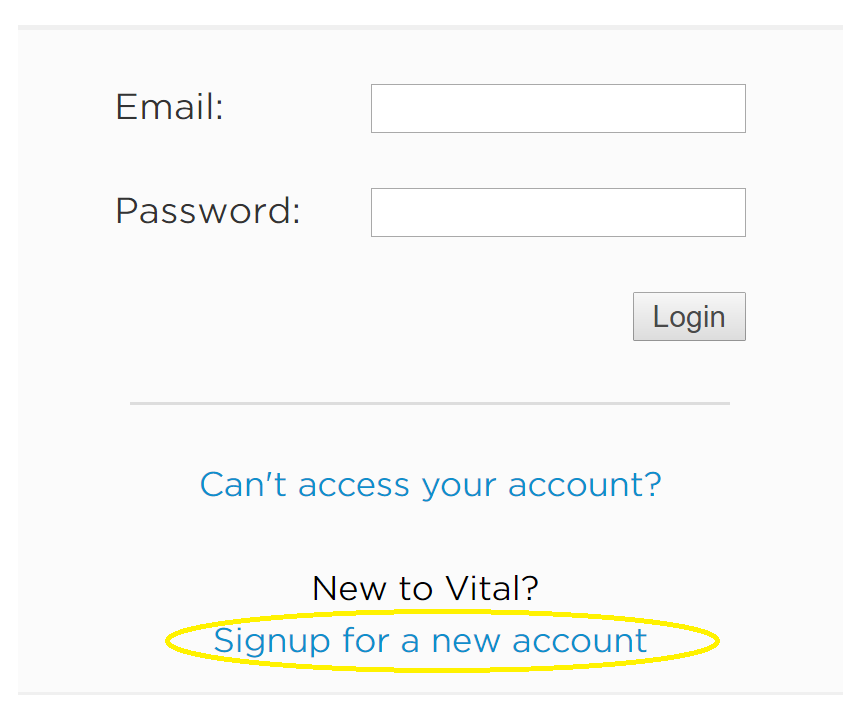
\includegraphics[scale=0.40]{account_creation.png}

}


You will be redirected to a page where you can submit your student information to receive a new account.

{%
\centering
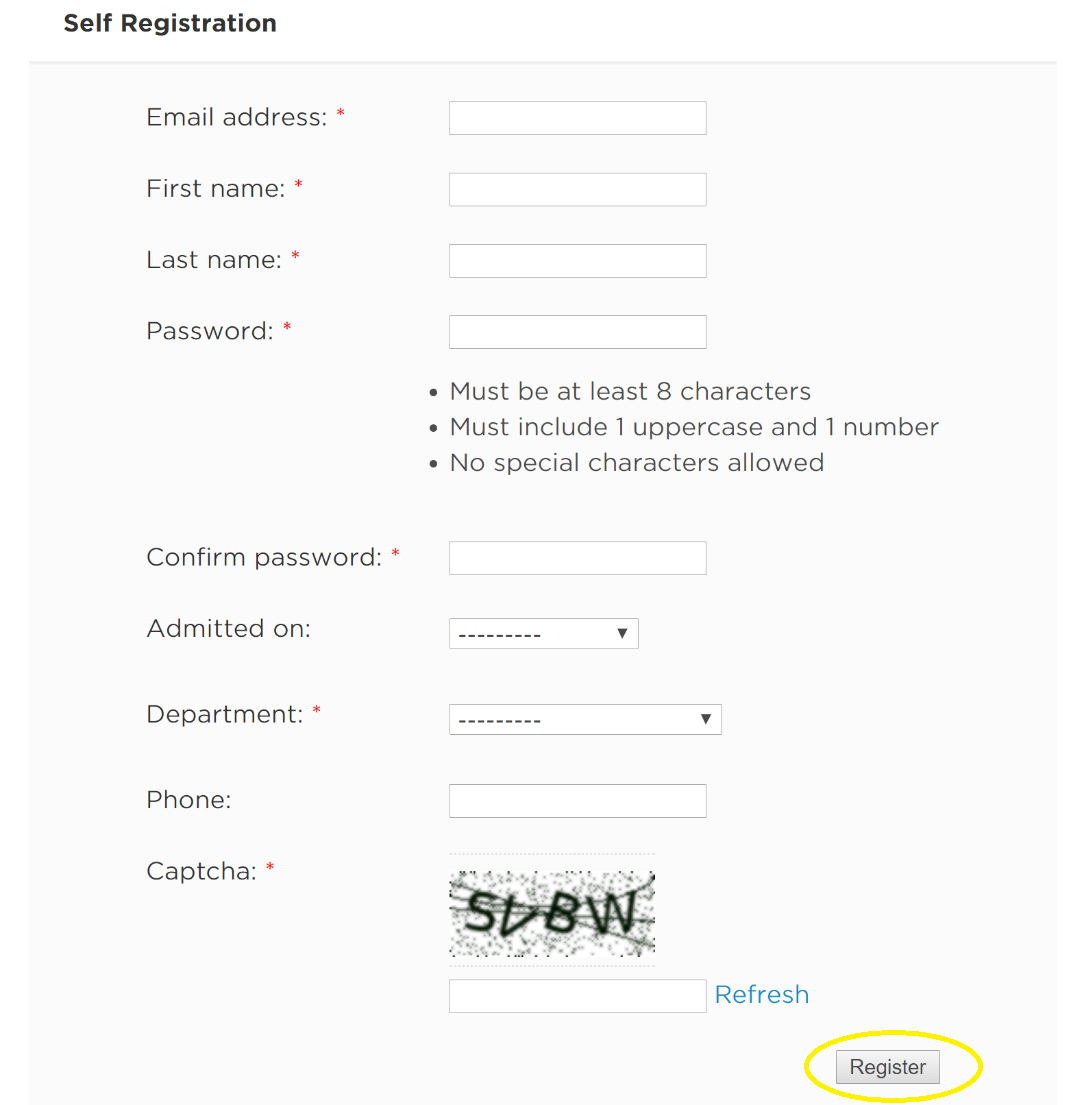
\includegraphics[scale=0.50]{self_registration.png}

}

When specifying a password, please be sure to meet the minimum complexity requirement. Do not reuse any password you may have already used for another system. Upon submitting this form, you will be directed back to the login page where you may authenticate to Vital with your new account.

\section*{Course Registration}
After you have created a Vital user account you will need to supply a registration code to get access to your course-specific lab environment. This code will be provided to you by your instructor.

Upon authenticating to Vital, you will be presented a page which contains links to your course lab environments. This list will appear empty if this is your first time registering for a course. You can add a course by clicking the ‘Add course’ link and providing your course registration code.
 
{%
\centering
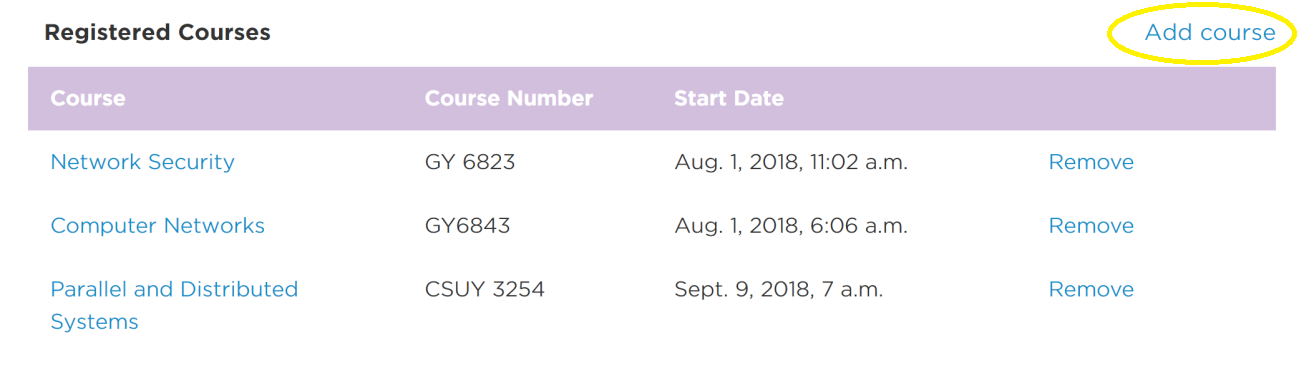
\includegraphics[scale=0.50]{course_registration.png}

}

\section*{Vital Features}
Now we are ready to get hands-on with some of the infrastructure provided to us by Vital. In this section we’ll examine the features of the platform and common best practices. 

Vital infrastructure always includes a default student account:

username: student\\
password: student

\subsection*{Course Environment}
Each course within Vital is unique. Certain course networks enable access to the Internet while others may be private. The virtual machines found within the course environment come equipped with applications you need to build and test your solutions.

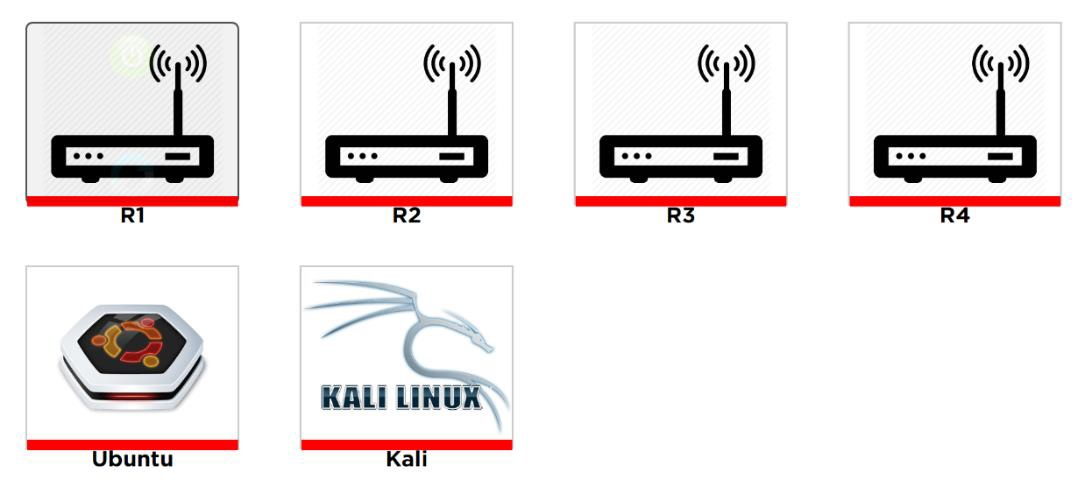
\includegraphics[scale=0.50]{course_environment}

As you can see in the image above, we are given access to six virtual machines in this particular course – Ubuntu, Kali Linux, and four routers.

\subsection*{Start and Stop Virtual Machines}
Machines with a red status bar on the course page are in an off state. If you place your mouse over any of the icons found within the course page, a green button will appear. 
Click this icon to start the virtual machine.

{%
\centering
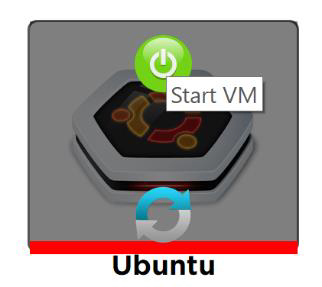
\includegraphics[scale=0.50]{start_vm.png}

}
After you have started the machine, the status bar will change to green to represent on and a new mouseover option, ‘View console’ will appear. Clicking the `view console’ icon will launch an interface.

{%
\centering
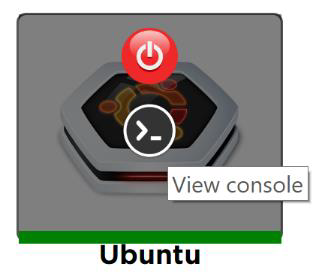
\includegraphics[scale=0.50]{view_console.png}

}
Notice that after starting the VM, the green power icon has changed to red. This can be used to turn the machine off.

After clicking `View console’ and logging in using the password student you will be presented the following interface (Ubuntu):

{%
\centering
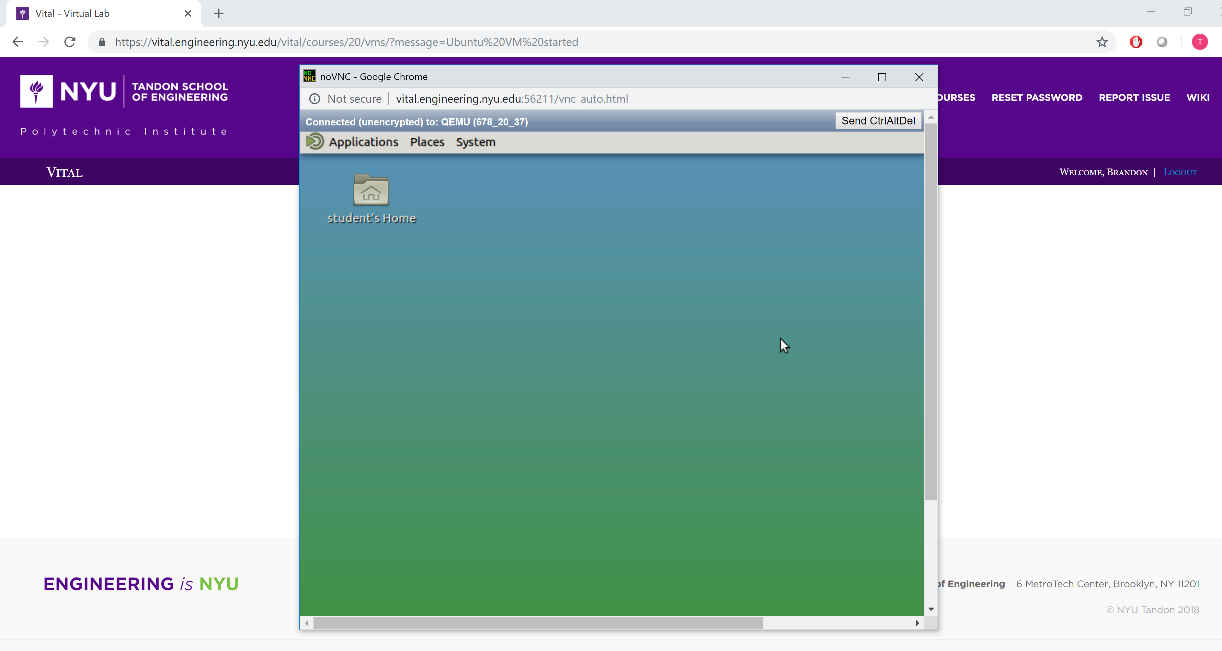
\includegraphics[scale=0.30]{vm_interface.png}

}

Do not forget to shut down all machines and log off Vital after completing lab assignments. Clicking the ‘Logout’ link in the upper-right corner will automatically send the shutdown signal to active machines. Leaving machines online for an extended period of time will result in a warning email.

\subsection*{Reimaging Virtual Machines}
While working on labs there may be situations where you want to restore a machine to its initial state. To accomplish this Vital gives students the option to reimage a virtual machine. This process will completely erase all user-specific data on the machine and restore it to its initial default settings. Data deleted this way cannot be recovered. Make sure you have saved your work elsewhere before initiating this process. You can reimage a machine by selecting the blue arrow mouseover option.

{%
\centering
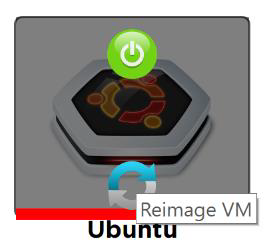
\includegraphics[scale=0.50]{reimage_vm.png}

}

\subsection*{SFTP File Transfers}
SSH File Transfer Protocol (SFTP) enables you to move files from one computer to another. You may need to do this for certain assignments. You must be on the NYU network or connected to the NYU VPN to resolve the domain name of the SFTP server (sftp.engineering.nyu.edu / 128.238.77.36). If you are not presently on the NYU network, skip to the section below for information on how to connect to the VPN.

Most operating systems come equipped with SFTP software which is accessible via the command line. You can authenticate to the SFTP server using your Vital username / password. 

For example:

\texttt{
> sftp <username>@sftp.engineering.nyu.edu
}

\texttt{
> <password>
}



After authenticating we can upload a file by executing:

\texttt{
sftp> put <path to file>
}

\texttt{
sftp> exit
}

{%
\centering
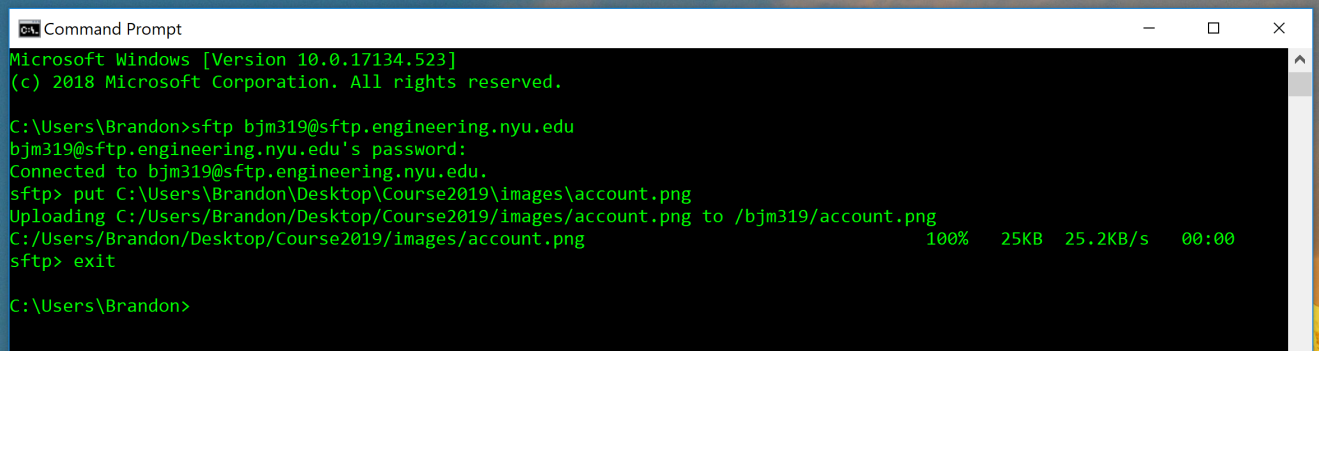
\includegraphics[width=\linewidth]{sftp1.png}

}


Once you have uploaded your files to the SFTP server, you can retrieve them from within the lab environment by executing the following commands:

\texttt{
> sftp <username>@sftp.engineering.nyu.edu
}

\texttt{
sftp> get <filename>
}

\texttt{
sftp> exit
}

{%
\centering
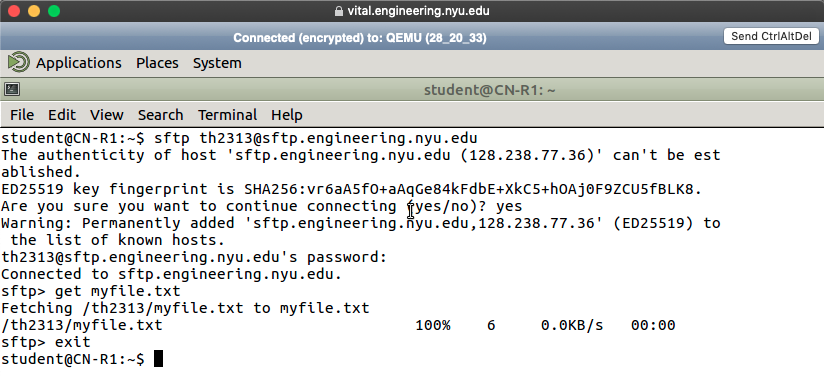
\includegraphics[width=\linewidth]{sftp2.png}

}

Once logged in to the SFTP server you can use the following command to see all options:

\texttt{
sftp> ?
}

\newpage

\section*{NYU VPN}
Download Cisco AnyConnect Client by clicking
\MYhref{https://www.cisco.com/c/en/us/support/security/anyconnect-secure-mobility-client/tsd-products-support-series-home.html}{here}.

Connect to the VPN by supplying vpn.nyu.edu and using two-factor authentication.

{%
\centering
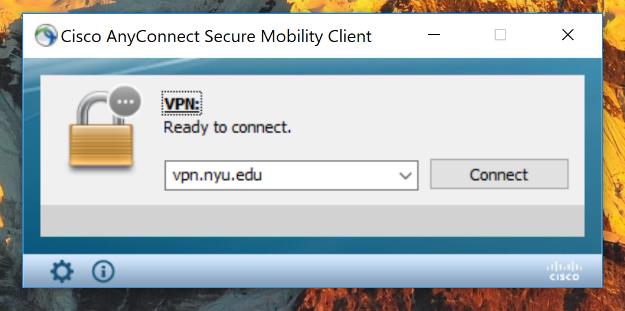
\includegraphics[scale=0.75]{vpn1.png}

}
After clicking `connect’ you will be prompted to authenticate. In the example below, the first password is an NYU account password. Scroll down and read the banner to provide a form of two-factor authentication for your second password.

{%
\centering
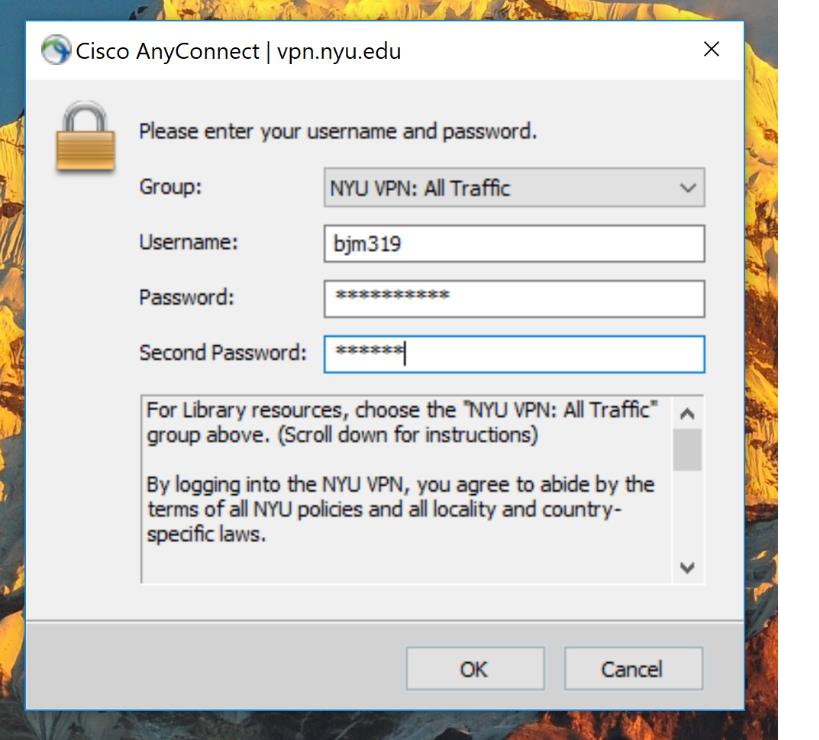
\includegraphics[scale=0.5]{vpn2.png}

}


\section*{Troubleshooting and Reporting Issues}
Please report any issues you may encounter while using Vital to our admin team at \\ \MYhref{mailto:vital@nyu.edu}{vital@nyu.edu}.

% --------------------------------------------------------------
%     You don't have to mess with anything below this line.
% --------------------------------------------------------------
 
\end{document}